\documentclass[12pt,a4paper]{article}
\usepackage[utf8]{inputenc}
\usepackage{amsmath}
\usepackage{amsfonts}
\usepackage{amssymb}
\usepackage{graphicx}
\usepackage[left=1cm,right=1cm,top=1cm,bottom=2cm]{geometry}
\usepackage{xcolor}
\usepackage{subcaption}
\usepackage{listings}
\usepackage{tabularx}
\usepackage{gensymb}
\usepackage{verbatim}
%\usepackage{subfig}
\usepackage{mathtools}
\usepackage{placeins}
\usepackage{float}

\usepackage{amsthm}
\usepackage{graphicx}
%\usepackage{subfigure}
\usepackage{algpseudocode}
\usepackage{algorithm}
\usepackage{bm}
\usepackage{bbm}
%\usepackage{kbordermatrix}
%\usepackage{mathdefs}
\usepackage{mathrsfs}
\usepackage{multirow}

\usepackage{hyperref}
\usepackage{cleveref}

\newtheorem{remark}{Remark}
\newtheorem{corollary}{Corollary}
\newtheorem{definition}{Definition}
\newtheorem{example}{Example}
\newtheorem{fact}{Fact}
\newtheorem{lemma}{Lemma}
\newtheorem{proposition}{Proposition}
\newtheorem{theorem}{Theorem}

\newcommand{\assref}[1]{Ass.~\ref{ass:#1}}
\newcommand{\clmref}[1]{Claim~\ref{clm:#1}}
\newcommand{\conref}[1]{Conj.~\ref{con:#1}}
\newcommand{\corref}[1]{Cor.~\ref{cor:#1}}
\newcommand{\defref}[1]{Def.~\ref{def:#1}}
\newcommand{\exaref}[1]{Ex.~\ref{exa:#1}}
\newcommand{\facref}[1]{Fact~\ref{fac:#1}}
\newcommand{\lemref}[1]{Lem.~\ref{lem:#1}}
\newcommand{\prpref}[1]{Prop.~\ref{prp:#1}}
\newcommand{\thmref}[1]{Thm.~\ref{thm:#1}}
\newcommand{\eqnref}[1]{(\ref{eq:#1})}
\newcommand{\secref}[1]{\S\ref{sec:#1}}
\newcommand{\appref}[1]{App.~\ref{app:#1}}
\newcommand{\figref}[1]{Fig.~\ref{fig:#1}}
\newcommand{\tabref}[1]{Table~\ref{tab:#1}}
\newcommand{\algoref}[1]{Alg.~\ref{alg:#1}}
\newcommand{\remref}[1]{Remark~\ref{rem:#1}}

\hypersetup{colorlinks=false}
\hypersetup{colorlinks,citecolor=black,filecolor=black,linkcolor=black,urlcolor=black}\label{sr_1}


\DeclarePairedDelimiter\ceil{\lceil}{\rceil}
\DeclarePairedDelimiter\floor{\lfloor}{\rfloor}

% disable indent
\setlength\parindent{0pt}

\title{Probability of Dice Sequences}
\author{Jonathan Stokes}

\begin{document}
\maketitle

\hrulefill\\

In rolling $6$ dice what is the probability of rolling $1,2,3,4$? Or more generally in rolling $n$ dice what is the probability for rolling a length $m$ sequence starting with $1$?
It is straight forward to estimate the probability of rolling these sequences using $100,000$ monte carlo simulations per dice count, see \cref{fig:monte_carlo_sim}.\\

\begin{figure}[H]
    \centering
    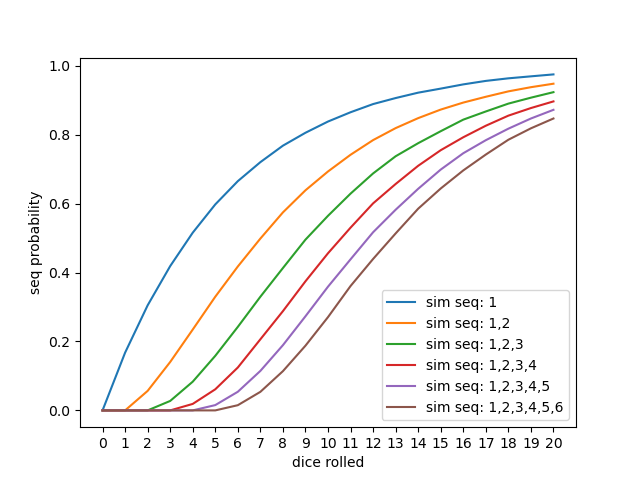
\includegraphics[width=0.5\textwidth]{figs/monte_carlo_seq_prob.png}
    \caption{Monte Carlo simulation of the probability of rolling different sequences starting at $1$ using $100,000$ rolls per dice count.}
    \label{fig:monte_carlo_sim}
\end{figure}

\hrulefill\\

At first this looks similar to the probability of drawing a straight in $5$ card draw poker. Lets define the event that one draws a straight in $5$ card draw poker
\begin{equation*}
A_5: \text{In drawing $5$ cards one draws a straight.}
\end{equation*}

If one draws a straight in $5$ card draw poker including a royal flush there are 

\begin{enumerate}
\item $\binom{10}{1}$ ways to choose the low card in the straight (recalling that the ace may be $1$ or follow the king). 
\item $\binom{4}{1}^5$ ways to select the card suits.
\end{enumerate}
and there are $\binom{52}{5}$ ways of drawing $5$ cards. So the probability of drawing the straight in $5$ card draw poker is
\begin{equation}
P(A_5) = \frac{\binom{10}{1}\binom{4}{1}^5}{\binom{52}{5}} \approx 0.00394
\end{equation}

Now lets define the more general event
\begin{equation*}
A_n: \text{In drawing $n$ cards one draws a straight.}
\end{equation*}

It follows that the probability of event $A_n$ for $n\in\{2 \ldots 13\}$ is 
\begin{equation}
P(A_n) = \frac{\binom{15-n}{1}\binom{4}{1}^n}{\binom{52}{n}}
\end{equation}

Now lets try applying the same reasoning to the probability of rolling a length $m$ sequence in a roll of $n$ dice for $n\geq m$ if we drop the requirement that the sequence starts at $1$. Lets define this event as
\begin{equation*}
A_{n,m}: \text{A length $m$ sequence appears in a roll of $n$ dice.}
\end{equation*}

Using the same reasoning as in drawing a straight of cards there are
\begin{enumerate}
\item $\binom{7-m}{1}$ ways to choose the low number in the sequence.
\item $\binom{6}{1}^{n-m}$ ways to roll the remaining dice.
\end{enumerate}
and there are $\binom{6}{1}^n$ ways of rolling $n$ dice. Therefore it would seem that the probability of rolling a length $m$ sequence in a roll of $n$ dice is,
\begin{equation}
P(A_{n,m}) = \frac{\binom{7-m}{1}\binom{6}{1}^{n-m}}{\binom{6}{1}^n} = \frac{\binom{7-m}{1}}{\binom{6}{1}^m} = \frac{7-m}{6^m}
\label{eq:wrong_eq}
\end{equation}
But looking at \cref{fig:monte_carlo_sim} this is clearly incorrect for $m=6$ and sequence $1,2,3,4,5,6$ as \cref{eq:wrong_eq} is constant in the number of dice rolled, $n$.\\

What did we do wrong? The term $\binom{7-m}{1}$ implicitly assumes that on any roll of the dice there are $6$ different numbers to choose from. In the case of cards this type of assumption is correct since every deck has $13$ distinct values ($14$ if the ace can be low and high). However in the case of a roll of $6$ dice we may not roll a $1$ leaving at most $5$ numbers to choose from in which case there are not $\binom{7-m}{1}$ ways to choose the lowest number in the sequence.\\

\hrulefill\\

So what is the solution? Lets start thinking about the case where $m=2$ and $n=3$. What is the probability of rolling a $1$ and a $2$ when rolling $3$ dice? First lets define the following events.
\begin{equation*}
A \text{: 1 appears in a roll of 3 dice.}
\end{equation*}
\begin{equation*}
B \text{: 2 appears in a roll of 3 dice.}
\end{equation*}

To find the probability of events $A$ and $B$ we need to find the probability of $\neg A$ and $\neg B$ which is the probability of rolling any of the other $5$ faces of the $3$ independent dice. Therefore
\begin{equation}
P(\neg A) = P(\neg B) = \left(\frac{5}{6}\right)^3
\label{eq:prob_not_one}
\end{equation}

and by analogy the probability of not rolling a $1$ and a $2$ is
\begin{equation}
P(\neg A \cap \neg B) = \left(\frac{4}{6}\right)^3
\label{eq:prob_one_and_two}
\end{equation}

It follows from \cref{eq:prob_not_one} that the probability of rolling either a $1$ or a $2$ is
\begin{equation}
P(A) = P(B) = 1-P(\neg A) = 1 - \left(\frac{5}{6}\right)^3 = \frac{91}{216}
\end{equation}
To answer our initial question above we need to find $P(A \cap B)$. Now the law of total probability states
\begin{equation}
P(A) = P(A|B)P(B)+P(A|\neg B)P(\neg B)
\label{eq:total_prob}
\end{equation}

Rearranging \cref{eq:total_prob} gives
\begin{equation}
P(A|B)  = \frac{P(A) - P(A|\neg B)P(\neg B)}{P(B)}\\
\end{equation}

Now since $P(A|\neg B) + P(\neg A|\neg B) = 1$ we can replace $P(A|\neg B)$ with $(1 - P(\neg A|\neg B))$ giving 
\begin{align}
P(A|B)  &= \frac{P(A) - (1 - P(\neg A|\neg B))P(\neg B)}{P(B)}
\label{eq:A_cond_B}
\end{align}

Notice it follows that
\begin{align}
P(A \cap B)     &= P(A|B)P(B)\\
                &= P(A) - (1 - P(\neg A|\neg B)) P(\neg B)\\
                &= P(A) - P(\neg B) + P(\neg A \cap \neg B)
\label{eq:reduced_A_and_B}
\end{align}
Plugging in the values above into \cref{eq:reduced_A_and_B} gives $P(A \cap B) \approx 0.139$.\\

Now given \cref{eq:reduced_A_and_B} does this generalize for $n\geq 2$ dice rolled? Lets first define the following events
\begin{equation}
A_n \text{: 1 appears in a roll of $n$ dice.}
\end{equation}
\begin{equation}
B_n \text{: 2 appears in a roll of $n$ dice.}
\end{equation}

\begin{align}
P(A_n \cap B_n) &= P(A_n) - P(\neg B_n) + P(\neg A_n \cap \neg B_n)\\
                &=  1-\left(\frac{5}{6}\right)^n -\left(\frac{5}{6}\right)^n + \left(\frac{4}{6}\right)^n\\
                &= 1 - 2\left(\frac{5}{6}\right)^n + \left(\frac{2}{3}\right)^n
\label{eq:A_and_B_sol}
\end{align}
and as $n\to\infty$, $P(A_n \cap B_n) \to 1$ as expected.\\

Can the solution above be generalized to the case of a length $m$ sequence? Lets first consider the case where $m=3$. In this case, by induction from \cref{eq:reduced_A_and_B} we write,\\

\begin{align}
P(A_n \cap B_n \cap C_n)    &= P(A_n) - P(\neg B_n) - P(\neg C_n)\\
                            &+ P(\neg A_n \cap \neg B_n) + P(\neg A_n \cap \neg C_n) + P(\neg B_n \cap \neg C_n)\\ 
                            &- P(\neg A_n \cap \neg B_n \cap \neg C_n)\\
                            &= 1 - 3\left(\frac{5}{6}\right)^n + 3\left(\frac{4}{6}\right)^n - \left(\frac{3}{6}\right)^n
\label{eq:A_and_B_and_C_sol}
\end{align}
\begin{figure}[H]
    \centering
    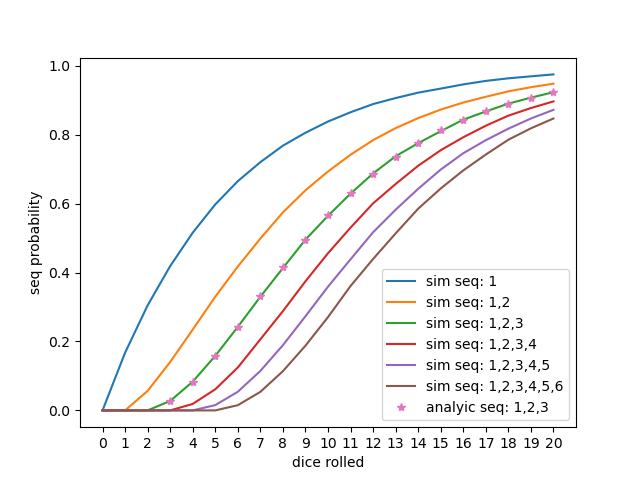
\includegraphics[width=0.5\textwidth]{figs/compare_analytic_sim.png}
    \caption{Plot of \cref{eq:A_and_B_and_C_sol}}
    \label{fig:compare_analytic_sim}
\end{figure}
\Cref{fig:compare_analytic_sim} compares the analytic solution given by \cref{eq:A_and_B_and_C_sol} with the simulated results. As expected they are similar.\\


Now we want an equation expressing the probability of rolling the sequence of dice $1$ to $m$ where $m\in\{1,2,3,4,5,6\}$. Given $n\geq m$ lets define the events
\begin{equation*}
A_{n,i} \text{: $i$ appears in a roll of $n$ dice.}
\end{equation*}
for $i \in \{1\ldots m\}$.\\

Now given \cref{eq:A_and_B_sol} and \cref{eq:A_and_B_and_C_sol} again by induction we can derive a closed form solution for the probability of a sequence of length $m$ starting at $1$ appearing in a given roll of dice as,
\begin{equation}
P\left(\bigcap_{i=0}^m A_{n,i}\right) = \sum_{i=0}^{m} (-1)^i \binom{m}{i}\left( \frac{6-i}{6} \right)^n
\label{eq:gen_sol}
\end{equation}

Using this equation to compute the analytic probability of rolling a dice sequence starting at $1$ of length $m$ and comparing these to the simulated results gives.

\begin{figure}[H]
    \centering
    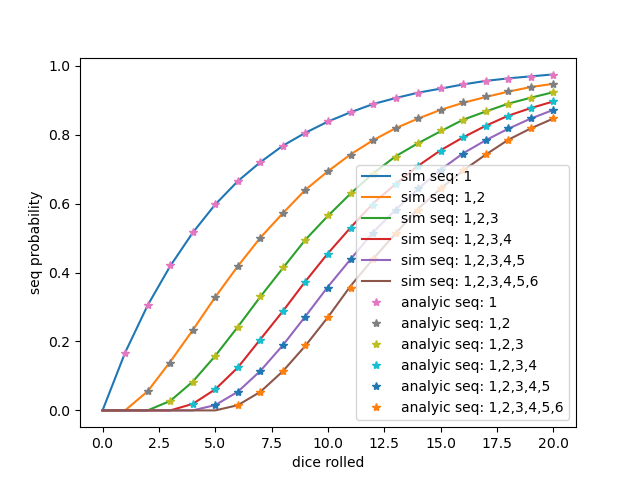
\includegraphics[width=0.5\textwidth]{figs/full_compare_analytic_sim.png}
    \caption{Plot of \cref{eq:gen_sol}}
    \label{fig:gen_sol}
\end{figure}

\end{document}
